\documentclass[11pt]{article}

\usepackage{amsmath}
\usepackage{graphicx}
\usepackage{multicol}
\usepackage{natbib}
\usepackage{wrapfig}
\usepackage{hyperref}
\usepackage{tabularx}
\usepackage{setspace}
\usepackage{comment}
\usepackage{color}
\usepackage[table]{xcolor}


\oddsidemargin 0cm
\evensidemargin 0cm

\usepackage{tocloft}

\setlength\cftparskip{6pt}
\setlength\cftbeforesecskip{4pt}
\setlength\cftaftertoctitleskip{2pt}

\usepackage[compact]{titlesec}  
\titlespacing{\section}{0pt}{0pt}{0pt}
\titlespacing{\subsection}{0pt}{0pt}{-5pt}
\titlespacing{\subsubsection}{0pt}{0pt}{-5pt}

\oddsidemargin 0cm
\evensidemargin 0cm

\usepackage[margin=1in]{geometry}


\parindent 0cm
\parskip 0.5cm

\linespread{1.1}

\usepackage{fancyhdr}
\pagestyle{plain}
%\fancyhf{}
%\fancyhead[L]{AOSS Reference Sheet}
%\fancyhead[CH]{test}
\fancyfoot[C]{Page \thepage}

\newcommand{\vb}{\mathbf}
\newcommand{\diff}[2]{\frac{d #1}{d #2}}
\newcommand{\diffsq}[2]{\frac{d^2 #1}{{d #2}^2}}
\newcommand{\pdiff}[2]{\frac{\partial #1}{\partial #2}}
\newcommand{\pdiffsq}[2]{\frac{\partial^2 #1}{{\partial #2}^2}}
\newcommand{\topic}{\textbf}
\newcommand{\arcsinh}{\mathrm{arcsinh}}
\newcommand{\arccosh}{\mathrm{arccosh}}
\newcommand{\arctanh}{\mathrm{arctanh}}

\renewcommand\refname{}

\begin{document}

\begin{center}
{\large \textbf{TempestExtremes: Indicators of change in the \\ characteristics of extreme weather}}

Dr. Paul Ullrich (PI) \\
\textit{Department of Land, Air and Water Resources, UC Davis}

Dr. Richard Grotjahn (Co-PI) \\
\textit{Department of Land, Air and Water Resources, UC Davis}

Dr. Colin Zarzycki (Co-I) \\
\textit{National Center for Atmospheric Research}
\end{center}

\begin{spacing}{-1.0}
\tableofcontents
\end{spacing}

\clearpage

\section{Scientific / Technical / Management}

\subsection{Motivation and Objectives}

This research proposal targets \textbf{NASA Strategic Research Objectives} (ROSES-2014) ``\textit{Climate Indicators and Data Products for Future National Climate Assessments}.''

The next century will see unprecedented changes to the climate system. These changes are particularly apparent to the general population via extreme weather events. The third National Climate Assessment (NCA) states ``changes in extreme weather and climate events, such as heat waves and droughts, are the primary way that most people experience climate change.'' The characteristics of extreme weather are key climate indicators, and addressing observed (lagging) and projected (leading) changes in these quantities will be important across multiple sectors, in multiple regions, and highly useful input to future NCAs.

Time series of the frequency, magnitude and other characteristics of extreme weather events over the past century are not well-measured. This project shall quantify climate change effects on a broad set of extreme weather events, including tropical cyclones (TCs), extratropical cyclones (ETCs), atmospheric blocks, atmospheric rivers, temperature extremes and precipitation extremes. 

The \textbf{central objective} of this proposal the provision of an assessment of trends in the \textbf{characteristics of extreme weather events} observed over the past century.  The \textbf{secondary objective} of this proposal is to provide a new \textbf{assessment capability} in the form of an \textbf{automated pipeline for detection and characterization of extreme weather events}.  These objectives are expanded as follows: 
\begin{itemize}
\item[(O1)] Identify and assess optimal detection and characterization algorithms for extreme weather events, including tropical cyclones, extratropical cyclones, atmospheric blocks, atmospheric rivers, extreme temperature and extreme precipitation events

\item[(O2)] Using reanalysis and model data in conjunction with the detection and characterization capability of (O1), provide an assessment of past changes in the characteristics of these extreme weather events.

\item[(O3)] Using large ensemble simulations from the Climate of the 20th Century (C20C) project, determine how the characteristics of extreme weather events under historical climate simulations differ from hypothetical climate simulations under preindustrial greenhouse gas concentrations.

%\item[O2] Using CMIP5 and CMIP6 model output, provide an assessment of predicted changes in the characteristics of extreme weather events.

\item[(O4)] Through the NASA Earth Exchange (NEX), provide scientists with the capability for automatic analysis of datasets using a suite of detection and characterization algorithms. 
\end{itemize}

%This work will emphasize regional and local-scale changes in extreme events.

\subsubsection{Central Theme: Extreme Weather}

This proposal targets a broad class of regional-scale \textbf{extreme weather} events that appear in climate datasets.  These events include both features that can be pinpointed at a particular global location, such as the sea-level pressure minimum associated with extratropical cyclones and tropical cyclones, and features that cover a region or area, including atmospheric rivers, atmospheric blocks, heat waves and precipitation extremes.  These events have both a limited spatial location / extent and a temporal component, including a distinct start and end time.  Extreme weather events include both propagating events (those that gradually change spatial position over time) and stationary events.  The \textbf{climate indicators} targeted by this proposal are the characteristics of these features, and are itemized in section \ref{sec:ExtremeWeather}.

The advantage of considering multiple extreme weather events under a single umbrella allows for analysis and identification of connections between these phenomena.  For instance, atmospheric blocking in the Eastern Pacific is responsible for redirecting atmospheric rivers, which in turn leads to a modification of precipitation patterns, a potential driver for a drought event.

According to the Intergovernmental Panel on Climate Change (IPCC), since 1980 annual losses from extreme weather events have ranged from several billion to over 200 billion.  Weather-related disasters have also caused a significant loss of human life over the past century, including nearly 500,000 deaths from the Bhola Cyclone in Bangladesh (1970), over 1,000,000 deaths from the 1931 central China floods, and 70,000 deaths from the European heat wave of 2003.  Consequently, understanding how extreme weather events have changed as a consequence of human influence is a pressing need of any climate assessment.

\subsubsection{Central Theme: Big Data}

The explosive growth in the number of observations and the rapidly increasing quantity of climate model output is a pressing challenge for climate researchers over the next decade \citep{levy2012bigdata}.  Multi-terabyte high-resolution spatiotemporal ensemble datasets are becoming the norm with data generation now rapidly outpacing the capacity for data analysis \citep{ganguly2008data}.  High-resolution global atmospheric simulations at scales of 10km will each require roughly a petabyte of active storage, and post-processing of this data will be an inevitable bottleneck in the process of understanding regional climate change.  The need for rapid high-throughput data analysis tools that have been validated on climate data is now greater than ever.  Current technologies include a smorgasbord of competing algorithms for detection and characterization that typically address only a single type of extreme weather, frequently require disparate input data formats and generally only work for data on a specific type of grid \citep{neu2013imilast}.  Consequently, this work has the potential to dramatically simplify and streamline the process of detection and characterization of synoptic scale phenomena in large-scale climate datasets, and so will lead to a better understanding of how these features are represented within climate simulations.  The TECA toolset \citep{PORSBKWFLMWWB2012PCS} aims to meet this need, although there is an outstanding need to develop the capacity of this toolset to answer questions on real meteorological phenomena.

%\subsubsection{Global Impact}

%This proposal aims to not only build on the previous work of the international community via integration of internationally developed datasets, but also aims to have a broad global impact.  Blocking events have been particularly disastrous throughout Europe and Russia in the past several decades (especially from the 2003 European heat wave and 2010 Russian heat wave), and global change threatens to worsen these events.  Extratropical cyclones have also been devastating, especially in northern Europe and the British Isles, but major storms associated with extratropical cyclones have also caused significant damage to New Zealand (1968) and Uruguay (2005).  Since this work focuses on leveraging high-throughput data analysis methods for global climate data, it is natural to consider these extreme events from a global perspective.  The results of this work will be shared with international collaborators in Europe and beyond, and will aid in developing effective mitigation and adaptation strategies against changing climate events.

%\subsubsection{Relevance}


\subsection{Extreme Weather Events} \label{sec:ExtremeWeather}

\subsubsection{Tropical Cyclones (TCs)}

Tropical cyclones (TCs) are severe storms originating in warm, tropical, ocean basins which are characterized by their strong surface winds and low pressure center. TCs are referred to regionally as tropical storms, hurricanes (Western Hemisphere) and typhoons (West Pacific). In other locales, they are also called cyclones or cyclonic storms. Storm sizes can range anywhere from 100 km to over 4,000 km in diameter. Landfalling TCs produce intense winds, heavy rain, high waves, and damaging storm surge in coastal locations \citep{EmanuelDivineWind}. They are currently estimated to be responsible for 19,000 fatalities per year and \$26 billion/year in damages worldwide \citep{Mendelsohn2012}, making them one of the most devastating natural phenomena.

Key sectors affected by tropical cyclones include energy, urban environments and transportation, primarily via infrastructural vulnerability.  Regions affected by TCs include the southwest, southeast and northeast, particularly along the coasts.

Key characteristics include wind intensity, radius of maximum wind, precipitation intensity, total overland precipitation and spatial distribution of tracks.

\subsubsection{Atmospheric blocking}

Sustained extreme temperatures, including heat waves and cold spells, which arise from atmospheric pressure blocking have been responsible for significant socioeconomic damage.  Historically, heat waves due to pressure blocking have led to thousands of deaths  in only the past decade, including roughly forty thousand casualties from the 2003 European heat wave \citep{bouchama20042003}, 220 deaths from the 2006 North American heat wave and over fifteen thousand casualties from the 2010 Russian heat wave.  In 2013, over 760 people died as a consequence of a long-running heat wave in Britain \citep{upi2013article}.  Additional losses from the North American heat wave were caused by drought conditions that spurred widespread forest fires, as well as large-scale convective storm events including the 2012 North American Derecho.  The economic cost of these events has been estimated to be in the tens of billions of dollars.

Blocking events, which arise from anomalous stationary pressure systems, are well characterized in the literature \citep{benzi1986anomalous}, and their connection with prolonged extreme temperatures is well known.  Using observations and model experiments, studies have shown that the duration of blocking events and associated heat waves may increase under global warming \citep{lupo1997climatological, beniston20042003}.  However, recent work by \cite{barnes2012methodology} observed that, using 500mb wind speed as an indicator and data from the CMIP5 dataset, duration of blocks remained roughly constant whereas frequency decreased.  Specific heat wave events have also been studied:  for instance, \cite{dole2011grl} use observational data to characterize human-induced influences on the 2010 Russian heat wave.  \cite{dandrea1998northern} compared atmospheric blocking events from 15 atmospheric general circulation models and found that models at the time tended to underestimate both blocking frequency and the average duration of blocks.  However, past studies do not address how the characteristics of general blocking events have been modified (or will be modified) by anthropogenic influences, and cannot state with statistical certainty how much the extreme heat wave events of the past decade can be attributed to human-induced changes.  The proposed work also leverages a large ensemble of previously unavailable climate simulations which are consistent with the observed and pre-industrial climate, and so has the potential to address the scientific questions in a rigorous statistical manner.

Key sectors affected by atmospheric blocking include water, energy, agriculture and human health.  In particular, persistent weather conditions caused by atmospheric blocks can affect precipitation patterns and lead to increases in local and regional air pollution.  Within the US, the northwest, southwest and Alaska are strongly affected by Pacific blocks which can redirect precipitation from the Pacific away from the coast.  The Great Plains, midwest, northeast and southeast are also affected by omega blocks, which are responsible for a range of extreme weather phenomena such as tornadoes and winter storms.

Key characteristics include intensity (for instance measured by the strength of the anomaly), duration and location.

\subsubsection{Extratropical Cyclones (ETCs)}

ETCs are phenomena associated with transient low-pressure systems occurring in the mid-latitudes of both hemispheres, can produce damaging levels of wind, precipitation, low temperatures, and flooding. In the span of a few hours, ETCs can travel across large areas and develop into massive storms resulting in widespread losses. Intense ETC events, such as the 1993 �Storm of the Century� in the eastern United States and the 1999 Windstorm Lothar in northern France, can cause hundreds of fatalities and significantly impact residential, commercial, and agricultural structures.

Extratropical cyclones are dominant features of the mid-latitude atmosphere associated with synoptic scale low pressure systems outside the tropics \citep{serreze1995climatological}.  Similar to tropical cyclones, these systems are responsible for high winds and extreme precipitation, and consequently have the potential for large socioeconomic impact \citep{ulbrich2009extra}.  Studies of extratropical cyclones under future climate scenarios suggest that the expansion of the Hadley circulation will drive extratropical cyclones poleward \citep{bengtsson2006storm} and the warmer climate will lead to an intensification of precipitation of these storms \citep{bengtsson2009will, zappa2013multi}.  This proposal aims to address the question of attribution of changes in ETCs to anthropogenic forcing, a question which has not yet been tackled in the literature.  It will also address the issue of whether observed intensification over the southern hemisphere in reanalysis data is corroborated with model results, or is likely associated with an increase in the number of observing stations \citep{simmonds2000variability}.

Key sectors affected by extratropical cyclones include energy, transportation, urban environments and human health.  Infrastructural vulnerabilities to extreme winter snowfall remains a persistent issue, but  cold temperatures and the effects of winter weather can also affect energy demand and human health.  Within the US, extratropical cyclones primarily affect the Northeast, Great Plains and Midwest regions.

Key characteristics include wind intensity, radius of maximum wind, precipitation intensity, total overland precipitation, proportion of precipitation as snowfall, and spatial distribution of tracks.

\subsubsection{Atmospheric Rivers (ARs)}

Atmospheric rivers are meteorological phenomena characterized by long, narrow plumes of increased atmospheric moisture stretching between the subtropics and the midlatitudes regions.  These features are responsible for 30\%-50\% of total US west coast precipitation, particularly during winter months, and 30\%-40\% of total seasonal snow water \citep{dettinger2011atmospheric}.  The majority of total seasonal snow water contribution from ARs will often occur as a result of 1-2 extreme AR events \citep{guan2010extreme}.  ARs are usually between 400 to 600\ km wide, and so at global model resolutions of $1^\circ$ are mostly unresolved, occupying as few as four grid cells in the latitudinal direction.

Key sectors affected by atmospheric rivers include water, energy and agriculture, particularly due to deposition of precipitation along the US West Coast.

Key characteristics include precipitation intensity and point of landfall.

\subsubsection{Extreme Heat Events (EHEs)}

{\color{red}[More from Richard here]}

Key sectors affected by extreme heat events include energy, agriculture and human health.  Energy infrastructure is particularly susceptible to extreme heat outbreaks, largely due to the increased energy demand required for air conditioning.  Extreme heat can also devastate crop yields and, in conjunction with high humidity, is a major cause of heat stroke and fatality among young children and the elderly, especially in disadvantaged communities.  All regions of the US are affected by extreme heat events.

Key characteristics include duration of heat events, apparent temperatures during heat events, overnight recovery temperatures and spatial extent.

\subsubsection{Extreme Precipitation Events (EPEs)}

{\color{red}[More from Richard here]}

Key sectors affected by extreme precipitation events include water, energy, transportation and agriculture.  All regions of the US are affected by extreme precipitation events.

Key characteristics include ...

%Key Historical NASA  NASA reanalysis products will be key to assess past changes, including the Modern Era Retrospective-analysis for Research and Applications (MERRA) and North American Regional Reanalysis (NARR) (for all extreme events), NASA Earth Exchange (NEX) Downscaled Climate Projections, Daymet reanalysis (for temperature and precipitation extremes) and PRISM precipitation data (for precipitation extremes).

\subsection{Datasets} \label{sec:Datasets}

\subsubsection{NARR} \label{sec:NARR}

\subsubsection{NEX Downscaled Climate Projections} \label{sec:NEXDownscaled}

\subsubsection{Daymet} \label{sec:DAYMET}

\subsubsection{PRISM} \label{sec:PRISM}

\subsubsection{MERRA} \label{sec:MERRA}

Reanalysis products represent climate model hindcasts which are tightly constrained to known observational data.  Development of these products has been a major research focus for a number of international groups, particularly over the past decade, with more than half a dozen agencies now maintaining reanalysis datasets.  However, these datasets have the potential to differ significantly depending on the choice of model, specific model parameters, the number of observations and the methodology by which data is assimilated into the model.  Although several major reanalysis products are available, this proposal aims to focus on results from NCEP \citep{kalnay1996ncep}, ERA-40 \citep{uppala2005era}, ERA-Interim \citep{simmons2007era}, MERRA \citep{rienecker2011merra} and C20C \citep{compo2011twentieth}.  For studying heat waves over the continental US, high resolution North American Regional Reanalysis (NARR) data will also be used.  The use of multiple datasets is important for identifying and overcoming biases associated with specific atmospheric models that may contaminate the results \citep{jun2008spatial}, and will lead to a set of more robust scientific conclusions.

\subsubsection{Climate of the 20th Century} \label{sec:EnsembleData}

As part of the Climate of the 20th Century (C20C) project, Michael Wehner, Da\'ith\'i Stone and others have performed 50 simulations of possible climate scenarios using historical sea-surface temperature (SST) forcings covering the period from 1959 to 2011 [\url{http://portal.nersc.gov/c20c/}].  Each of these simulations represent one possible atmosphere that is consistent with known historical greenhouse gas emissions and ocean temperatures.  A further ensemble of 50 simulations have been computed using historical data which has been adjusted to remove anthropogenic forcing, including greenhouse gas emissions and warming of SSTs, to mimic the state of the pre-industrial atmosphere.  These two ensembles are commonly referred to as ``the world that was'' and ``the world that could have been.''  The goal of the proposed project is to leverage these datasets to better understand the role that humans have played in affecting regional and global climate over the past century.

\subsubsection{CLIVAR Experiments} \label{sec:CLIVAR}

Climate Variability and Predictability (CLIVAR) experiments are commonly used to isolate changes in the climate system associated with accepted forcing mechanisms.  Specifically, the experiments of interest for this proposal use present-day forcing which has been modified by (a) doubling atmospheric CO2 concentration (2xCO2), (b) increasing global sea-surface temperatures by 2 degrees (SST+2) or (c) a combination of (a) and (b).  CLIVAR runs have been completed using CESM over a 14-17 year integration period at 25km and a 24-27 year integration period at 100km and are now available for analysis.

\subsubsection{IPCC/CMIP5} \label{sec:IPCC-CMIP5}

The fifth Climate Model Intercomparison Project (CMIP5) represents a major international collaboration, having brought together 19 global Earth-system models from the around the world to better understand the effect of changing climate over the next century.  These experiments use a standard suite of four Representative Concentration Pathways (RCPs) to account for predicted changes in greenhouse gas emissions, and are performed at horizontal resolutions ranging from 25km to 200km.  Results from the multi-model ensemble are now available for scientific analysis.  Specifically, this proposal will analyze the results of this ensemble to develop a consensus and understanding of how the community of climate models predict pressure blocking events/heat waves and extratropical cyclones and understand how CESM compares to other models so as to better isolate its model biases.

\subsection{Methods} \label{sec:Methods}

This proposal will investigate and intercompare detection criteria for extreme weather events to identify the best algorithm for automated detection to identify relevant characteristics.

The capability to address such a wide array of extremes hinges on the TempestExtremes software package, a new suite of flexible detection and characterization algorithms developed by the PI for processing large climate datasets. This package uses an algorithmic framework known as ``MapReduce'' to first detect candidate events at individual times using specified criteria. Stitching is then used to assess the evolution of related detections over time. The result is an objective calculation of the climate indicator that can be automated and parallelized for multiple datasets.

\subsubsection{Tropical cyclones and extratropical cyclones}

In addition to intense winds and low surface pressures, tropical cyclones are characterized by a strong local maximum in cyclonic vorticity and an upper-level warm core. The latter arises from strong diabetic processes in the center of the storm which release large quantities of latent heat via condensational warming. This results a local horizontal maximum in temperature between 4 and 14 kilometers above the surface \citep{SternNolan2011}. The vast majority of existing tropical cyclone detection algorithms identify storms on a time-independent basis based on some combination of collocated sea level pressure minimum, low-level vorticity maximum, and upper-level temperature maximum (e.g., \citet{Vitart1997,Oouchi2006,Bengtsson2007a,Knutson2007,Walsh2007,Tory2013a,Zarzycki2014AMIPTCs}). Detected candidates which are close in both space and time are stitched together to form trajectories. Wind speeds associated with each storm are then used to isolate systems considered intense enough to fit the standard definition of tropical cyclones. While the minimum sustained surface wind speed for a system to be defined by the World Meteorological Organization is 17.5 m/s, this threshold is frequently modified when assessing climate date for reasons such as insufficient resolution to model intense tropical cyclones and different heights where the wind measurement is assessed \citep{Walsh2007}.

Atmospheric reanalysis data will be used in conjunction with the International Best Track Archive for Climate Stewardship (IBTrACS) tropical cyclone best track database \citep{Knapp2010} to assess the performance of commonly-used tracking parameter combinations. Sensitivity tests which perturb the thresholds used to define tropical cyclones in climate data will be completed to assess whether or not the storm detection process is highly sensitive to the choice of specific criteria.

Detection algorithms for ETCs have been proposed by \cite{wang2006climatology}, \cite{wernli2006surface}, \cite{raible2008northern} and others (see, for example, the review paper by \cite{ulbrich2009extra}) using a combination of variables, including 850 hPa wind speed, vorticity, sea level pressure, precipitation, geopotential and upper-level temperature.  Accurate detection of ETCs over high topography remains an outstanding question that will be addressed with this work.  Again a number of approaches will be studied and tuned using a suite of reanalysis data, and verified using multiple datasets and a visual intercomparison.  In particular, we will verify that historically relevant extratropical storms are correctly detected and characterized by the algorithm.

In TempestExtremes, detection of both ETCs and TCs is handled by first searching for minima in the sea-level pressure field.  Thresholds can then be specified on the pointwise Laplacian of pressure, maximum or minimum latitude and topographic height at the point of detection.  Additional criteria are also available, including requirement or elimination of candidates based on the presence of a warm core aloft (detected as a maximum in the temperature field at 200hPa and 500hPa within a specified distance), the presence of a relative vorticity maximum within a specified distance, or the presence of a closed pressure contour.  Once candidate storms have been identified, stitching of candidates to form cyclone tracks is performed.  The stitching algorithm provides options for distance between candidate points in time, minimum track duration, minimum distance between begin and endpoint, minimum path length, as well as other user-specified thresholds on quantities such as windspeed or surface pressure.  The stitching algorithm also provides an option for identifying trajectories with detection gaps, for example when candidates are present at times 1,2,3,5,6, and 7.  These criteria amalgamate a wide range of detection and stitching algorithms specified in the literature {\color{red}[references from Colin]}.

%Preliminary results from TECA using a composite scheme and ETC density plot are shown in Figure \ref{fig:ETCDetection} for a sample CESM CLIVAR dataset.

Recently, the IMILAST project \citep{neu2013imilast} has been conceived as a grand-scale international intercomparison effort of ETC detection algorithms.  Although all of the detection algorithms were run on the ERA-Interim dataset, dramatic variability was observed between total counts of ETCs over the analysis period by different algorithms.  Consistency between detection methods was observed to occur largely for deep, strong ETCs.  These results again suggest that detection of ETCs may require a comprehensive approach that uses multiple detection criteria to identify candidate storms.  This proposal will also extend upon the work of IMILAST by studying the capability of detection algorithms to successfully detect and characterize ETCs in NCEP reanalysis, 20th Century reanalysis and alternative climatologies, all of which are expected to be more representative of typical CESM simulation results.  This proposal will further compare how ETC statistics differ between these datasets, and whether climate signals are robust across ETC detection algorithms.

This task aims to perform the first comprehensive study of blocking events and ETCs in historical reanalyses data, including the NCEP, ERA-40, MERRA and C20C datasets.  Using the detection algorithms developed in Task 1, this proposal aims to determine historical counts of blocking events / ETCs and differences between the event characteristics obtained from each reanalysis dataset.  A particular focus in this analysis will be given to extreme value statistics (how does the return time of extreme blocking events vary by region), which are associated with blocking events / ETCs that have the potential for the most socioeconomic damage.  Properties specific to blocking events that will be considered include intensity, duration, classification, return time and associated weather.  Those specific to ETCs include wind intensity (in terms of vorticity, minimum sea-level pressure or gradient of sea-level pressure), radius of maximum winds, intensity of precipitation, latitude of genesis point, latitude of termination and probability of transit beyond a given latitude.  This task will tackle the question of how these characteristics can be filtered from each dataset once a successful detection has been obtained.  To do so, this work will rely on both past surveys of event characteristics \citep{serreze1995climatological}, as well as building an understanding of the general features of ETCs in historical reanalysis data.

Note that differences in the statistics of ETCs between the ERA-40 and NCEP reanalyses have been previously examined by \cite{hodges2003comparison}, \cite{wang2006climatology} and \cite{raible2008northern}. They observed significant differences in these datasets -- notably the ERA reanalysis generally produced stronger ETCs in both extratropical regions, although this result was especially pronounced in the austral extratropics. It was also observed that track length also appeared to be longer in the ERA-40 dataset.  Given the observed variation of 50\% or more in precipitation, these differences could have a significant effect on policy decisions.

\subsubsection{Atmospheric blocks}

This proposal aims to compare two algorithmic approaches for identifying and characterizing atmospheric blocking events.  Formally, atmospheric blocking is a meteorological phenomenon defined by an anti-cyclonic quasi-stationary high-pressure system persisting for several days to weeks and so is associated with negative vorticity anomalies in the Northern hemisphere (positive in the Southern hemisphere) and positive geopotential perturbation.  Blocks must also be tracked in time to verify persistence, requiring the use of the two-pronged approach that underlies the MapReduce algorithm.  Various algorithms have been developed for the identification of blocking events in atmospheric model data \citep{tibaldi1990operational, wiedenmann2002climatology, pelly2003new, scherrer2006two, tyrlis2008aspects, barriopedro2010application, barnes2012methodology}, and most of these approaches use either geopotential height, 500mb velocity or potential vorticity as indicators (with a variety of thresholds).  However, robust algorithmic detection of atmospheric blocking events has been particularly difficult due to the fact that atmospheric blocking manifests in many different forms \citep{haby2008blocking}, such as Rex Blocks, Omega Blocks, etc.  Notably, the focus of the majority of past studies has also been on Euro-Atlantic blocking.  Consequently, it is anticipated that global detection of blocking events will require a multi-pronged approach.  In order to manage all sets of input data, a combination of processing methods using Python scripts and C++ will be used for handling of reanalysis data and CESM output.  Idealized tests to verify correct behavior of this algorithm will use the idealized baroclinic instability test with potential vorticity tracer proposed by \cite{JPWCJJKRBR2013QJRMS}.  Each detection algorithm will be applied to the reanalysis datasets to determine which formulation provides the most robust approach for detection of both northern hemisphere and southern hemisphere blocking events.  Preliminary results showing regions of anti-cyclonic column-integrated potential vorticity (PV) anomalies using a detection approach analogous to \cite{scherrer2006two} are shown in Figure \ref{fig:BlockingDetection}.

\begin{figure}
\begin{center}
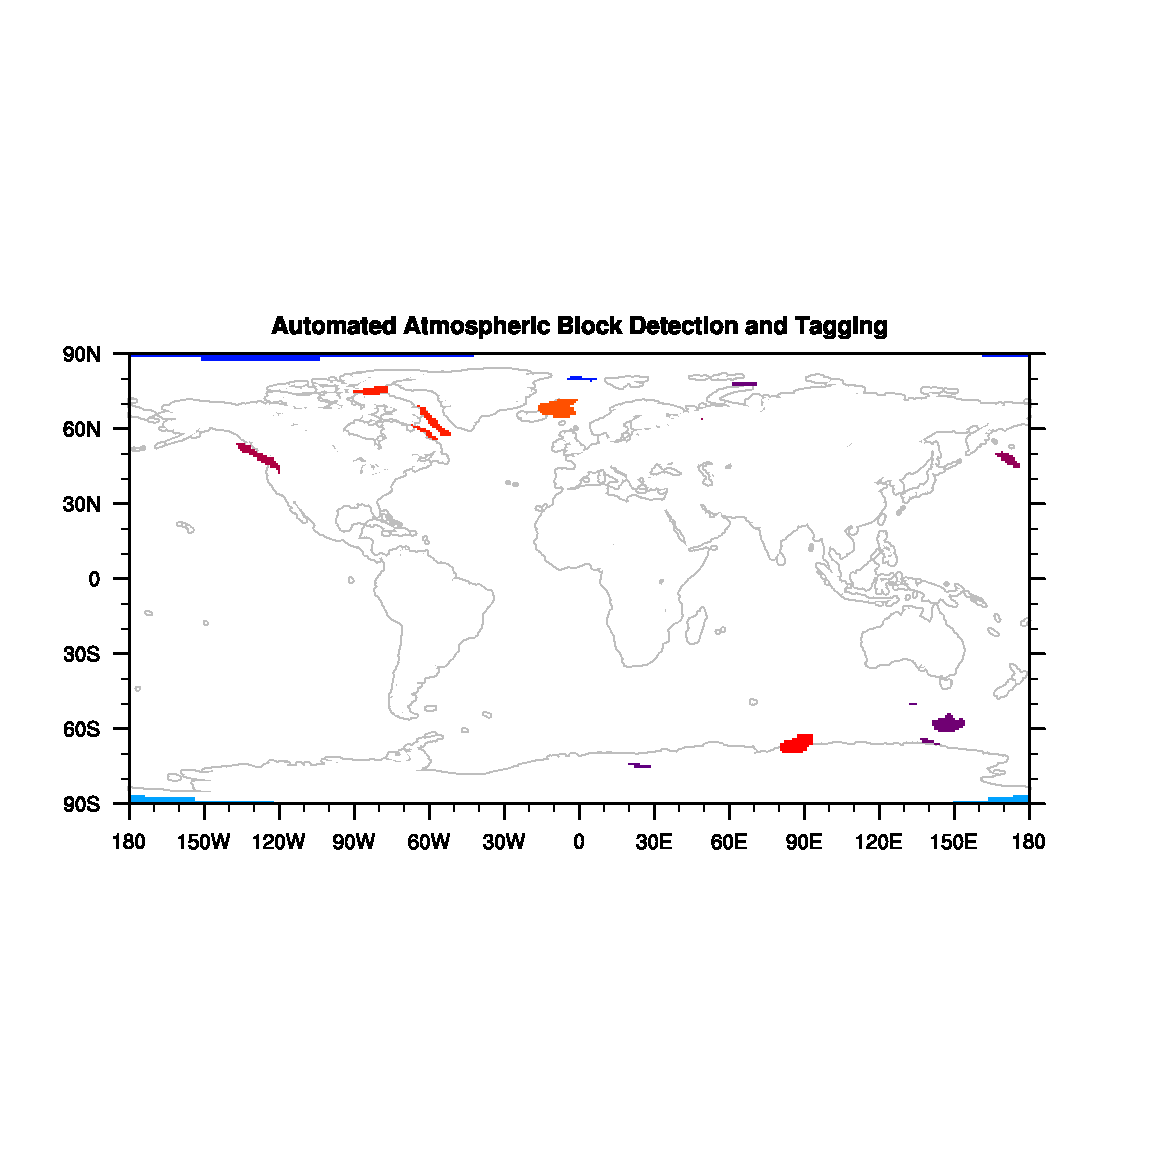
\includegraphics[width=6.5in]{blob_plot}
\end{center}
\caption{Anti-cyclonic column-integrated potential vorticity (PV) anomalies (against a 15 year monthly averaged background state taken from 1979 to 1993), identifying regions where the column integrated PV is less than $-1.3$ PVU (northern hemisphere) and greater than $+1.3$ PVU (southern hemisphere).  This criteria for blocking event detection is described by \cite{scherrer2006two}, as applied to the ERA-Interim reanalysis data for 11 June 2005.  Discrete blocking events are tagged with a unique identifier based on spatial and temporal connectivity.} \label{fig:BlockingDetection}
\end{figure}

\subsubsection{Atmospheric rivers}

This proposal will develop, implement and analyze automated atmospheric river detection and characterization for understanding AR events in the variable-resolution data \citep{ralph2004satellite, lavers2012detection}.  The characterization of atmospheric rivers will be based on \cite{neiman2008meteorological} and \cite{guan2010extreme}, who use column-integrated water vapor to identify filamentary structures over the eastern Pacific.  The capability to detect these structures will utilize technology from the TempestExtremes software package, a new suite of flexible detection and characterization algorithms developed by the PI for processing large climate datasets.  AR structures will be agglomerated in space using a graph traversal algorithm, and then connected in time by determining overlaps in detections at adjacent time points.  Discrete AR events will then be characterized in terms of point of landfall and total associated precipitation (rainfall and snowfall).  Statistics will then be computed on these quantities including proportion of precipitation associated with AR events, frequency of AR events and mean spatial point of landfall.  This information will then be used for addressing both sensitivity of AR events to grid resolution (using 110km, 28km and 14km datasets) and changes to AR events under future climatology.

\subsubsection{Temperature extremes}

{\color{red}[More from Richard]}

This task seeks to implement and analyze several algorithmic approaches for the detection and characterization of heat waves and cold spells.  Part of the goal of this work will be to determine if detection indicators of heat waves are correlated with typical indicators for blocking events in the reanalysis datasets.  An analogous study was performed \cite{della2007summer}, which examined summer heat waves over western Europe over the 20th century and showed that many European heat waves are correlated with anomalous high pressure systems over Scandinavia characteristic of an atmospheric blocking event.  This proposal aims to expand this study to the global scale using the previously developed framework of multiple reanalysis datasets and detection algorithms.

\subsubsection{Precipitation extremes}

{\color{red}[More from Richard]}

This task seeks to implement and analyze several algorithmic approaches for the detection and characterization of precipitation extremes, including droughts and flooding.

\subsubsection{Human Attribution}

This proposal will apply an analogous detection procedure on the ensemble of ``world that could have been'' simulations.  Since this second set of simulations arise from a world without anthropogenic forcing, differences in the statistics of blocking events and ETCs can be effectively attributed to anthropogenic drivers.  Consequently, this study aims to look at how the statistics of blocking events have changed under human influence (such a study is known as detection and attribution).

The results of this task would also provide enlightenment on specific atmospheric events of the past (other such studies include \cite{stott2004human} and \cite{pall2011anthropogenic}).  Namely, it would address questions such as ``what was the probability of the 1993 Storm of the Century in a world with and without anthropogenic forcing?''  Statistically significant differences between the probability in the forced and unforced simulations in 1993 would lead to conclusions on the influence of human activity on the likelihood of these events.  The large ensemble (50 members) that will be leveraged as part of this project is necessary in order to provide accurate statistics on relatively infrequent events such as these, and so this proposal is uniquely positioned to answer these questions.

\subsection{Research Tasks}

%\subsubsection{Climate Indicators}

%This project will provide an assessment of changes in many of the characteristics of extreme weather events.  Under this umbrella we include an assessment from key NASA datasets, plus two projects ``assessing human-induced climate change'' and ``projecting future change.''

%To support future assessment capabilities, this project further seeks to integrate the TempestExtremes package in the NASA Earth Exchange (NEX) to allow for high-throughput analysis of submitted datasets from other NEX users.

\subsubsection{(T1) Detection and characterization of ARs, Heat and Precip.}

This research task will implement detection and characterization algorithms for atmospheric rivers, heat extremes and precipitation extremes in TempestExtremes.

\begin{tabular}{ccc}
\hline Extreme & Methods & Status \\
\hline ETCs and TCs & Various SLP-based & {\color{green} Implemented} \\
Blocking & \cite{scherrer2006two}, \cite{pelly2003new} & {\color{green} Implemented} \\
ARs & \cite{neiman2008meteorological} & {\color{red} To be implemented} \\
Heat & ? & {\color{red} To be implemented} \\
Precip. & ? & {\color{red} To be implemented} \\
\hline
\end{tabular}

\subsubsection{(T2) Assessment of lagging indicators}

The climate indicator focus of this proposal will assess past trends in the characteristics of extreme weather events that have been enumerated in section \ref{sec:ExtremeWeather}.  NASA reanalysis products described in section \ref{sec:Datasets} will be key to assess past changes, including the Modern Era Retrospective-analysis for Research and Applications (MERRA) and North American Regional Reanalysis (NARR) (for all extreme events), NASA Earth Exchange (NEX) Downscaled Climate Projections, Daymet reanalysis (for temperature and precipitation extremes) and PRISM precipitation data (for precipitation extremes).

\subsubsection{(T3) Assessing Human-Induced Climate Change}

The question of the influence human activity on the frequency and magnitude of extreme weather events of the past decade has remained largely unanswered.

As part of the Climate of the 20th Century (C20C) project, 100 climate simulations have been produced covering the period 1959-2011, half representing a climate consistent with known greenhouse gas emissions and sea-surface temperatures, and half representing conditions with anthropogenic forcing removed.  By contrasting extreme weather events within these two datasets, anthropogenic influences can be separated from natural variability. These ensemble runs enlarge the sample of extreme events, which are inherently rare. Hence these data are particularly useful when statistically analyzing the time series of observation-based historical data and improving estimates of probability distributions useful to various application sectors.

\subsubsection{(T4) Assessment of leading indicators (future change)}

Two options are available for providing projections of future change: static climatologies produced via Climate Variability and Predictability (CLIVAR) experiments under doubled atmospheric CO$_2$ and/or increased sea-surface temperatures, and dynamic climatologies obtained from the CMIP5 multi-model multi-ensemble database.

\subsubsection{(T5) Integration of the Extreme Weather Pipeline in NEX}

\begin{figure}
\begin{center}
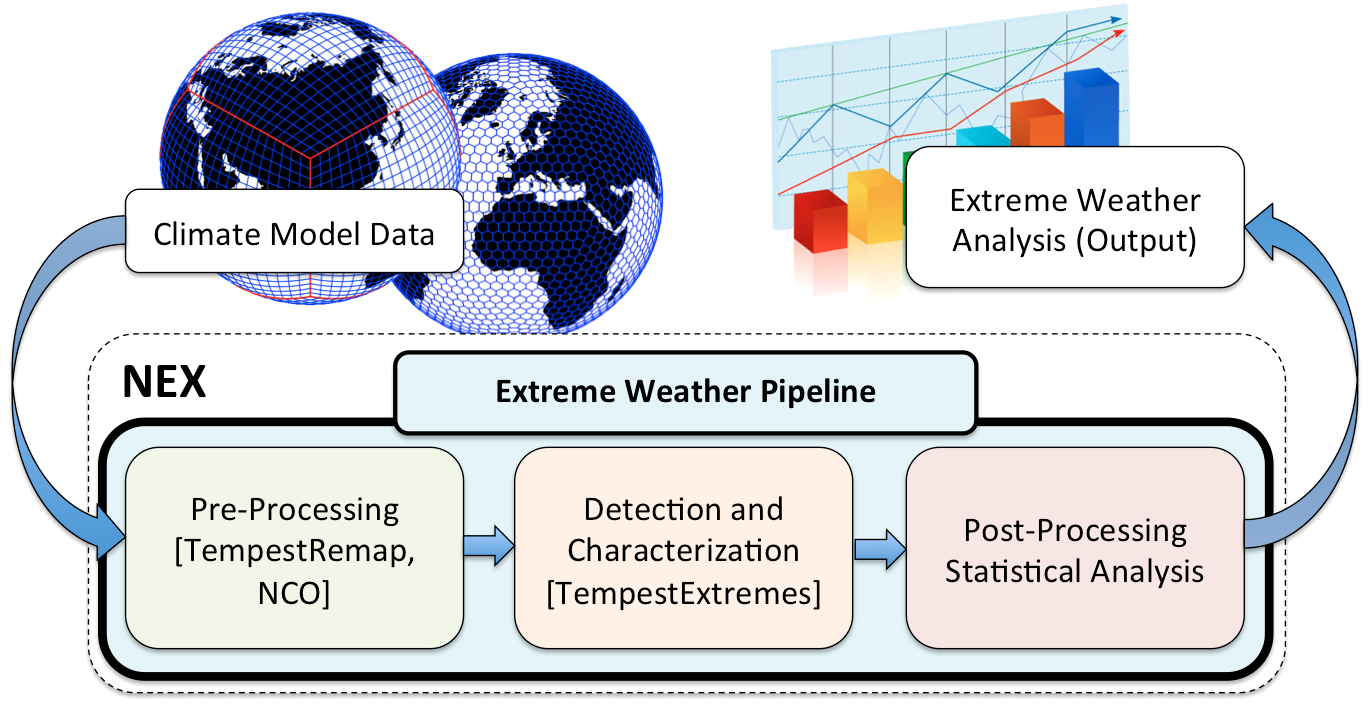
\includegraphics[width=5in]{TempestPipeline.png}
\end{center}
\caption{A depiction of the Extreme Weather Pipeline for supporting analysis of climate data through the NEX system.} \label{fig:TempestPipeline}
\end{figure}

We propose the integration of the TempestExtremes detection and characterization software into the existing NASA Earth Exchange (NEX) infrastructure, to provide a capability for scientists to quickly obtain information and statistics on extreme weather events from their climate datasets.  A depiction of the software pipeline exposed to climate scientists is shown in Figure \ref{fig:TempestPipeline}.  First, gridded climate data and grid metadata are provided to the pre-processor so as to convert the data to a format compatible with the detection and characterization toolset.  This step entails both regridding of the climate data to a latitude-longitude grid and computation of additional diagnostic variables (for instance, computation of vorticity from wind vectors).  The processed input data is then fed into the detection and characterization software (TempestExtremes), where the user has the capability to specify the set of extreme weather events to identify and their characteristics (indicators) of interest.  Multiple detection algorithms (even for the same extreme weather event) or parameter choices can be specified at this stage.  The results of the detection and characterization step is then fed into a statistical post-processor, where the user again has the option of computing statistical quantities of interest.

The software associated with this proposal will be implemented using C++.  Execution of the code will be performed on NASA's computing systems via the NEX interface.

\subsubsection{Visualization}

\section{Timetable of Activities and Management Plan} \label{sec:Timeline}

Each of the graduate student researchers involved in this project will work on two of the atmospheric features presented in this proposal, although it is anticipated that there will be substantial collaboration on the technical level.  PI Ullrich will be in charge of coordinating software development and ensuring that this work meets the necessary software engineering guidelines.  The approximate timeline of the research component of this proposal is as follows:

The first year will be dedicated towards development of detection and characterization algorithms (Task 1 and 2), debugging of the suite of detection tools and post-processing of reanalysis data to ensure compatibility with TECA.  After an initial understanding of these phenomena has been developed, construction of the idealized test cases will begin (Task 3).  The second year will focus on validation and verification of the toolset, including detection and correlation of heat wave events and atmospheric blocks, and evaluation of model performance relative to reanalysis data (Task 4).  During this year work will also begin on the detection and attribution study, using the CESM ensemble data at all resolutions to verify consistency with the reanalysis data and the development of idealized test cases (Task 5).  Work on using CLIVAR ensemble datasets to predict changes in ETCs and blocking events during Year 2, including investigation of tropical cyclones undergoing the extratropical transition (Task 6).  The third year will focus on the IPCC/CMIP5 datasets to determine future predictions on how the qualities of atmospheric blocking events will be modified by the changing climate (Task  6).  This timeline is summarized in Table \ref{tab:ExpectedTimeline}.

\begin{table}
\begin{tabular}{c||c|c|c|c||c|c|c|c||c|c|c|c|}
& \multicolumn{4}{c}{Year 1} & \multicolumn{4}{c}{Year 2} & \multicolumn{4}{c}{Year 3}  \\
  \hline
         & 1st & 2nd & 3rd & 4th & 1st & 2nd & 3rd & 4th  & 1st & 2nd & 3rd & 4th \\
\hline
\hline
Detection algorithm dev. & \cellcolor{red!35} & \cellcolor{red!35} & \cellcolor{red!35} & \cellcolor{red!35} & & & & & & & &  \\
\hline
Characterization dev. & \cellcolor{blue!35} & \cellcolor{blue!35} & \cellcolor{blue!35} & \cellcolor{blue!35} & & & & & & & &  \\
\hline
Reanalysis data  & \cellcolor{cyan!35} & \cellcolor{cyan!35} & \cellcolor{cyan!35} &  \cellcolor{cyan!35}  & \cellcolor{cyan!35} & \cellcolor{cyan!35} & & & & & & \\
\hline
Validation / Verification  & & & & & \cellcolor{red!35} & \cellcolor{red!35} & \cellcolor{red!35} &  \cellcolor{red!35}  & & & & \\
\hline
Detection / Attribution & & & & & \cellcolor{blue!35} & \cellcolor{blue!35} & \cellcolor{blue!35} &  \cellcolor{blue!35}  & \cellcolor{blue!35} & \cellcolor{blue!35} & & \\
\hline
Predictive study (static)  & & & & & & & \cellcolor{cyan!35} &  \cellcolor{cyan!35}  & \cellcolor{cyan!35} & \cellcolor{cyan!35} & \cellcolor{cyan!35} &  \cellcolor{cyan!35} \\
\hline
Predictive study (dynamic)  & & & & & & & & & \cellcolor{green!35} & \cellcolor{green!35} & \cellcolor{green!35} &  \cellcolor{green!35} \\
  \hline
\end{tabular}
\caption{Expected timeline of (split in quarters for each year) for all major activities.} \label{tab:ExpectedTimeline}
\end{table}

We anticipate that multiple major peer-reviewed publications will arise from this work, addressing the studies of detection, attribution and prediction. Further, this work will be presented at major scientific meetings, including the annual meetings for the American Meteorological Society, the European Geophysical Union and the American Geophysical Union.  A final report will be developed as part of this proposal summarizing the conclusions drawn from this work along with advice for future work that could target model improvements in CESM, and possible future research directions.

\section{Bibliography and References Cited}

\vspace{-1cm}
\bibliography{Ullrich-NASAIndicators-Bibliography}
\bibliographystyle{wileyqj}

\clearpage

\end{document}
